\documentclass{article}

\usepackage{fancyhdr}
\usepackage{extramarks}
\usepackage{amsmath}
\usepackage{amsthm}
\usepackage{amsfonts}
\usepackage{amssymb}
\usepackage{xparse}
\usepackage{tikz}
\usepackage{graphicx}
\usepackage[plain]{algorithm}
\usepackage{algpseudocode}
\usepackage{listings}
\usepackage{hyperref}
\usepackage[per-mode = fraction]{siunitx}
\usepackage{calc}

\usetikzlibrary{automata,positioning}

\hypersetup{
    colorlinks=true,
    linkcolor=blue,
    filecolor=magenta,
    urlcolor=blue,
    }

\urlstyle{same}

%
% Basic Document Settings
%

\topmargin=-0.45in
\evensidemargin=0in
\oddsidemargin=0in
\textwidth=6.5in
\textheight=9.0in
\headsep=0.25in

\linespread{1.1}

\pagestyle{fancy}
\lhead{\hmwkAuthorName}
\chead{\hmwkClass\ (\hmwkClassInstructor,\ \hmwkClassTime): \hmwkTitle}
\rhead{\firstxmark}
\lfoot{\lastxmark}
\cfoot{\thepage}

\renewcommand\headrulewidth{0.4pt}
\renewcommand\footrulewidth{0.4pt}

\setlength\parindent{0pt}
\allowdisplaybreaks
%
% Title Page
%

\title{
	\vspace{2in}
	\textmd{\textbf{\hmwkClass:\ \hmwkTitle}}\\
	\normalsize\vspace{0.1in}\small{Due\ on\ \hmwkDueDate\ at \hmwkDueTime}\\
	\vspace{0.1in}\large{\textit{\hmwkClassInstructor,\ \hmwkClassTime}}
	\vspace{3in}
}
\author{\textbf{\hmwkAuthorName}}
\date{\hmwkCompletionDate}

%
% Create Problem Sections
%

\newcommand{\enterProblemHeader}[1]{
	\nobreak\extramarks{}{Problem #1 continued on next page\ldots}\nobreak{}
	\nobreak\extramarks{Problem #1 (continued)}{Problem #1 continued on next page\ldots}\nobreak{}
}

\newcommand{\exitProblemHeader}[1]{
	\nobreak\extramarks{Problem #1 (continued)}{Problem #1 continued on next page\ldots}\nobreak{}
	\nobreak\extramarks{Problem #1}{}\nobreak{}
}

%
% Homework Problem Environment
%
\NewDocumentEnvironment{hwkProblem}{m m s}{
	\section*{Problem #1: #2}
	\enterProblemHeader{#1}
	\setcounter{partCounter}{1}
}{
	\exitProblemHeader{#1}
	\IfBooleanF{#3} % if star, no new page
		{\newpage}
}

% Alias for the Solution section header
\newcommand{\hwkSol}{\vspace{\baselineskip / 2}\textbf{\Large Solution}\vspace{\baselineskip / 2}}

% Alias for the Solution Part subsection header
\newcounter{partCounter}
\newcommand{\hwkPart}{
	\vspace{\baselineskip / 2}
	\textbf{\large Part \Alph{partCounter}}
	\vspace{\baselineskip / 2}
	\stepcounter{partCounter}
}

%
% Various Helper Commands
%

% Such That
\newcommand{\st}{\text{s.t.}}

% Useful for algorithms
\newcommand{\alg}[1]{\textsc{\bfseries \footnotesize #1}}

% For derivatives
\newcommand{\deriv}[1]{\frac{\mathrm{d}}{\mathrm{d}x} (#1)}

% For partial derivatives
\newcommand{\pderiv}[2]{\frac{\partial}{\partial #1} (#2)}

% Integral dx
\newcommand{\dx}{\mathrm{d}x}
\newcommand{\dy}{\mathrm{d}y}

% Probability commands: Expectation, Variance, Covariance, Bias
\newcommand{\e}[1]{\mathrm{e}#1}
\newcommand{\E}{\mathrm{E}}
\newcommand{\Var}{\mathrm{Var}}
\newcommand{\Cov}{\mathrm{Cov}}
\newcommand{\Bias}{\mathrm{Bias}}

% Defining Units that are not in the SI base
\DeclareSIUnit\bar{bar}
\DeclareSIUnit\ft{ft}
\DeclareSIUnit\dollar{\$}
\DeclareSIUnit\cent{\text{\textcent}}
\DeclareSIUnit\c{\degreeCelsius}

% Code Listing config
\usepackage{xcolor}
\definecolor{codegreen}{rgb}{0,0.6,0}
\definecolor{codegray}{rgb}{0.5,0.5,0.5}
\definecolor{codepurple}{rgb}{0.58,0,0.82}
\definecolor{backcolour}{rgb}{0.95,0.95,0.92}
\lstdefinestyle{overleaf}{
	% backgroundcolor=\color{backcolour},
	commentstyle=\color{codegreen},
	keywordstyle=\color{magenta},
	numberstyle=\tiny\color{codegray},
	stringstyle=\color{codepurple},
	basicstyle=\ttfamily\footnotesize,
	breakatwhitespace=false,
	breaklines=true,
	captionpos=b,
	keepspaces=true,
	numbers=left,
	numbersep=5pt,
	showspaces=false,
	showstringspaces=false,
	showtabs=false,
	tabsize=4
}

\usepackage[latte]{catppuccinpalette}
\lstdefinestyle{catppuccin}{
	breaklines=true,
	keepspaces=true,
	numbers=left,
	numbersep=5pt,
	showspaces=false,
	showstringspaces=false,
	breakatwhitespace=true,
	tabsize=4,
	stringstyle = {\color{CtpGreen}},
	commentstyle={\color{CtpOverlay1}},
	basicstyle = {\small\color{CtpText}\ttfamily},
	keywordstyle = {\color{CtpMauve}},
	keywordstyle = [2]{\color{CtpBlue}},
	keywordstyle = [3]{\color{CtpYellow}},
	keywordstyle = [4]{\color{CtpLavender}},
	keywordstyle = [5]{\color{CtpPeach}},
	keywordstyle = [6]{\color{CtpTeal}}
}

\lstset{style=catppuccin}


%
% Homework Details
%   - Title
%   - Subtitle
%   - Due date
%   - Due time
%   - Course
%   - Section/Time
%   - Instructor
%   - Author
%

\newcommand{\hmwkTitle}{Homework 03}
\newcommand{\hmwkSubTitle}{Ground Tracks}
\newcommand{\hmwkDueDate}{March 13, 2025}
\newcommand{\hmwkDueTime}{09:30 AM}
\newcommand{\hmwkClass}{ENAE 404 - 0101}
\newcommand{\hmwkClassTime}{09:30}
\newcommand{\hmwkClassInstructor}{Dr. Barbee}
\newcommand{\hmwkAuthorName}{\textbf{Vai Srivastava}}
\newcommand{\hmwkCompletionDate}{\today}

\begin{document}

\maketitle

\pagebreak

\begin{hwkProblem}{1}{}

	Conceptual questions:
	\begin{enumerate}
		\item Give the semi-major axis, eccentricity and inclination of an orbit whose ground track is a point.
		\item Explain why argment of periapsis equal to \qty{0}{\degree} or \qty{180}{\degree} produces equatorial symmetry.
		\item Consider the Molniya orbit. Which one orbital element would you change so that the spacecraft would spend a long time veiewing the Southern hemisphere (rather than the Northern hemisphere)? Identify the orbital element and the value of this orbital element that would preserve the same structure of the ground track (just flipped to observe the Southern hemisphere).
	\end{enumerate}

	\hwkSol

	\hwkPart

	For an orbit whose ground track is a fixed point, the spacecraft must be in a geostationary orbit. This requires:
	\begin{align*}
		a &\approx \qty{42164}{\km} \quad (\text{from Earth’s center}), \\
		e &= 0 \quad (\text{circular orbit}), \\
		i &= \qty{0}{\degree} \quad (\text{orbit in the equatorial plane}).
	\end{align*}

	\hwkPart

	The argument of periapsis, \( \omega \), defines the orientation of the ellipse within the orbital plane relative to the line of nodes. When \( \omega \) is \qty{0}{\degree} or \qty{180}{\degree}, the line of apsides is aligned with the line of nodes. This alignment causes the orbit to be symmetric about the equatorial plane.

	\hwkPart

	A standard Molniya orbit is designed with an argument of periapsis \( \omega \approx \qty{270}{\degree} \) so that the apogee is in the Northern Hemisphere. To flip the ground track so that the apogee is over the Southern Hemisphere, one would change the argument of periapsis to \( \omega = \qty{90}{\degree} \).

\end{hwkProblem}
\begin{hwkProblem}{2}{}

	Plot one day ground tracks for the following orbits:
	\begin{center}
		\begin{tabular}{cccccc}
			\hline Spacecraft ID & \( \mathrm{a}(\unit{\km}) \) & e   & \( \mathrm{i}(\unit{\degree}) \) & \( \Omega(\unit{\degree}) \) & \( \omega(\unit{\degree}) \) \\
			\hline
			A                    & 42164                        & 0.3 & 40                               & 0                            & 0                            \\
			B                    & 26562                        & 0.3 & 40                               & 0                            & 0                            \\
			C                    & 42164                        & 0.3 & 60                               & 0                            & 70                           \\
			D                    & 42164                        & 0.3 & 30                               & 0                            & 70                           \\
			E                    & 42164                        & 0.3 & 120                              & 0                            & 0                            \\
			\hline
		\end{tabular}
	\end{center}
	Compare and contrast the ground track for Orbit E to that of Orbit A.

	\hwkSol
	
	\lstinputlisting[language=python, caption={P02 Python Code}, label={lst:s02}]{./code/s02.py}

	\hwkPart

	\begin{figure}[H]
		\begin{center}
			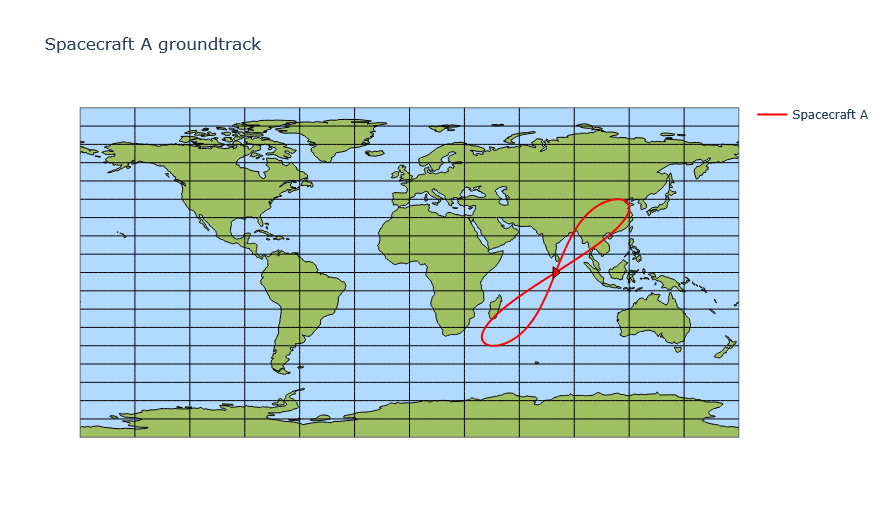
\includegraphics[width=0.85\textwidth]{./images/s02a.png}
		\end{center}
		\caption{Spacecraft A groundtrack}\label{fig:s02a}
	\end{figure}

	\lstinputlisting[language=python, caption={P02a Python Code}, label={lst:s02a}]{./code/s02a.py}

	\hwkPart

	\begin{figure}[H]
		\begin{center}
			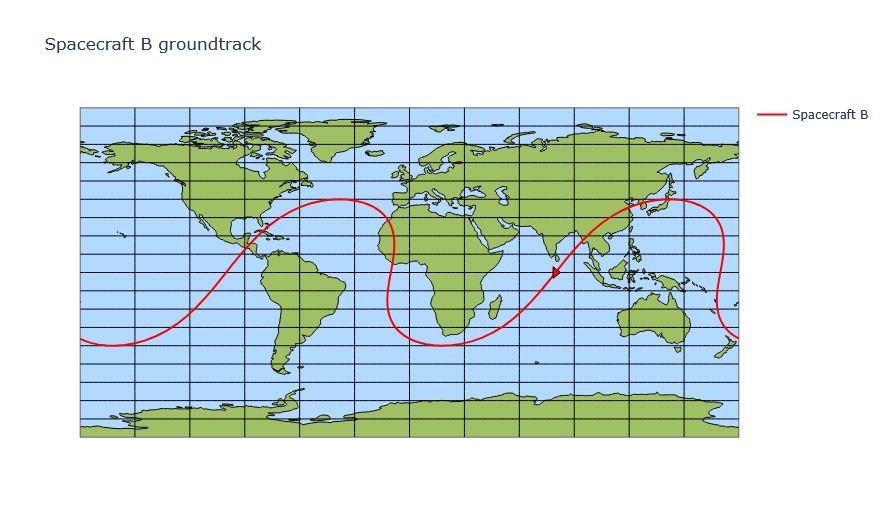
\includegraphics[width=0.85\textwidth]{./images/s02b.png}
		\end{center}
		\caption{Spacecraft B groundtrack}\label{fig:s02b}
	\end{figure}

	\lstinputlisting[language=python, caption={P02b Python Code}, label={lst:s02b}]{./code/s02b.py}

	\hwkPart

	\begin{figure}[H]
		\begin{center}
			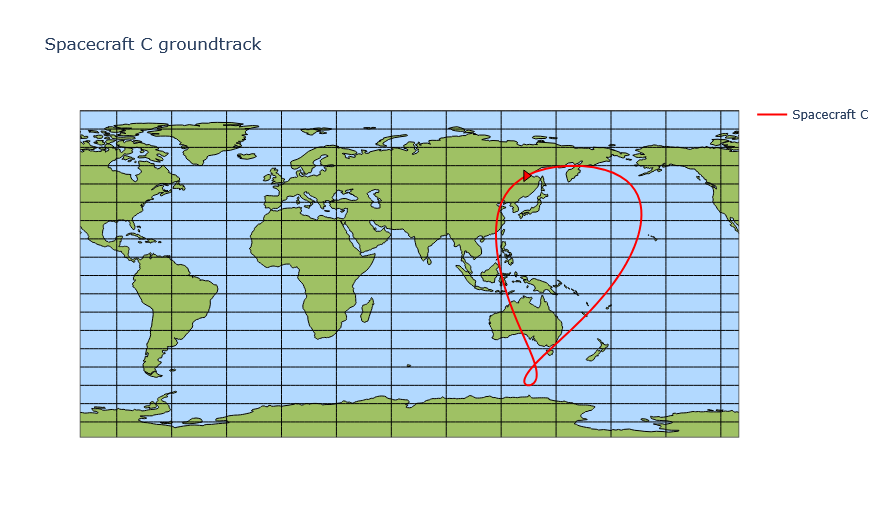
\includegraphics[width=0.85\textwidth]{./images/s02c.png}
		\end{center}
		\caption{Spacecraft C groundtrack}\label{fig:s02c}
	\end{figure}

	\lstinputlisting[language=python, caption={P02c Python Code}, label={lst:s02c}]{./code/s02c.py}

	\hwkPart

	\begin{figure}[H]
		\begin{center}
			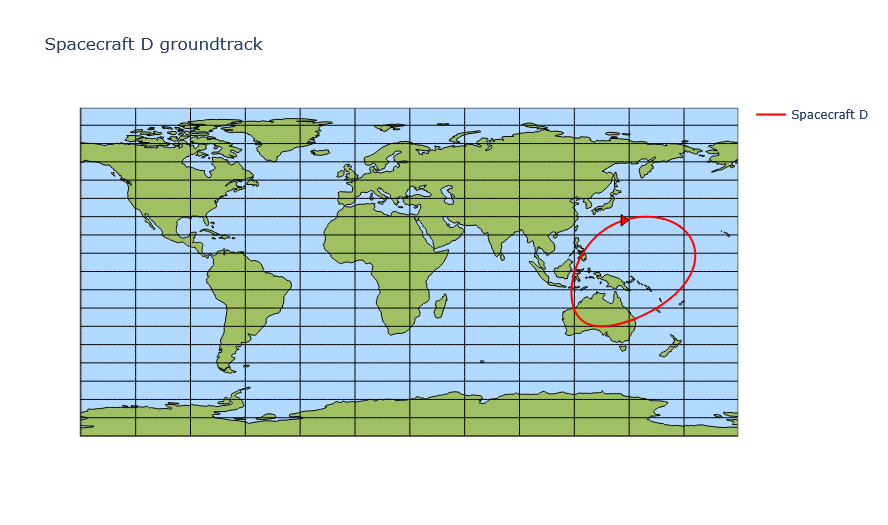
\includegraphics[width=0.85\textwidth]{./images/s02d.png}
		\end{center}
		\caption{Spacecraft D groundtrack}\label{fig:s02d}
	\end{figure}

	\lstinputlisting[language=python, caption={P02d Python Code}, label={lst:s02d}]{./code/s02d.py}

	\hwkPart

	\begin{figure}[H]
		\begin{center}
			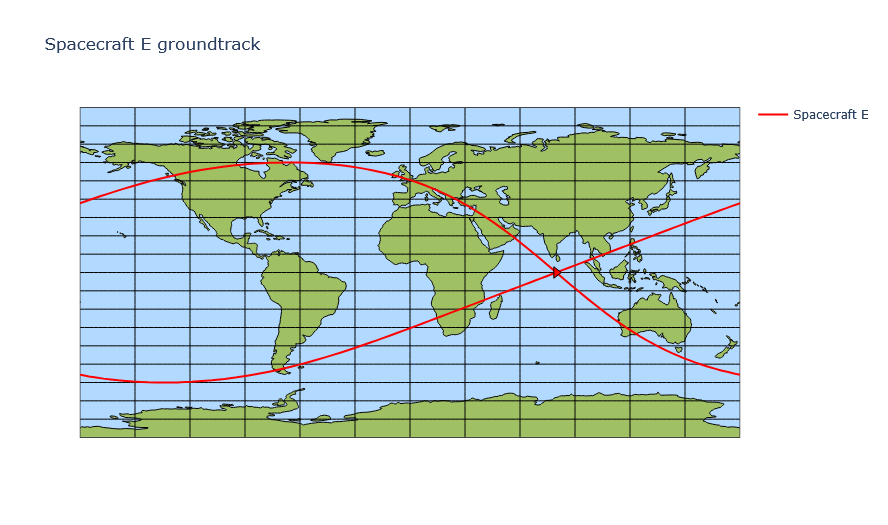
\includegraphics[width=0.85\textwidth]{./images/s02e.png}
		\end{center}
		\caption{Spacecraft E groundtrack}\label{fig:s02e}
	\end{figure}

	\lstinputlisting[language=python, caption={P02e Python Code}, label={lst:s02e}]{./code/s02e.py}

	\hwkPart

	The ground tracks for orbits A and E have the same lemniscate shape, though their rotation and scale are vastly different. The similarity is due to A and E sharing many orbital elements, though the differences are due to the varied inclination angle between the two orbits.

\end{hwkProblem}
\begin{hwkProblem}{3}{}

	Calculate the \( \Delta \mathrm{V} \) required to execute a Hohmann transfer from a circular orbit with radius \qty{14e3}{\km} to a circular orbit with radius \qty{8e3}{\km}. Assume the central body is the Earth. State whether the maneuvers increase or decrease the spacecraft's velocity.

	\hwkSol

	\begin{align*}
		a_t &= \frac{r_1 + r_2}{2} = \frac{\SI{14000}{\km} + \SI{8000}{\km}}{2} \\
		      &= \qty{11000}{\km} \\
		v_{c_{1}} &= \sqrt{\frac{\mu}{r_1}} = \sqrt{\frac{398600}{14000}} \\
                                       &\approx \qty{5.34}{\km\per\s} \\
		v_{t_{1}} &= \sqrt{\mu\left(\frac{2}{r_1} - \frac{1}{a_t}\right)} = \sqrt{398600\left(\frac{2}{14000} - \frac{1}{11000}\right)} \\
			 &\approx \SI{4.55}{\km/s} \\
              	\Delta v_1 &= v_{c_{1}} - v_{t_{1}} \approx \qty{5.34}{\km\per\s} - \qty{4.55}{\km\per\s} \\
                                       &= \qty{0.79}{\km\per\s} \\
		v_{c_{2}} &= \sqrt{\frac{\mu}{r_2}} = \sqrt{\frac{398600}{8000}} \\
                                 &\approx \qty{7.06}{\km\per\s} \\
		v_{t_{2}} &= \sqrt{\mu\left(\frac{2}{r_2} - \frac{1}{a_t}\right)} = \sqrt{398600\left(\frac{2}{8000} - \frac{1}{11000}\right)} \\
			 &\approx \qty{7.97}{\km\per\s} \\
		\Delta v_2 &= v_{t_{2}} - v_{c_{2}} \approx \qty{7.97}{\km\per\s} - \qty{7.06}{\km\per\s} \\
                                       &= \qty{0.91}{\km\per\s} \\
		\Delta v_{\text{total}} &= \Delta v_1 + \Delta v_2 \approx \qty{0.79}{\km\per\s} + \qty{0.91}{\km\per\s} \\ 
		\Delta v_{\text{total}} &= \qty{1.70}{\km\per\s} \quad \qed
	\end{align*}
	The Hohmann transfer requires a total \( \Delta \mathrm{V} \approx \qty{1.70}{\km\per\s} \). Both maneuvers decrease the spacecraft's velocity.

\end{hwkProblem}
\end{document}
